\documentclass[11pt,oneside,a4paper]{article} %% oneside and NOT twoside here !!
% http://www-h.eng.cam.ac.uk/help/tpl/textprocessing/latex_maths+pix/node6.html symboles de math
% http://fr.wikibooks.org/wiki/Programmation_LaTeX Programmation latex (wikibook)
%=========================== En-Tete =================================
%--- Insertion de paquetages (optionnel) ---
\usepackage[french]{babel}
\usepackage{a4}	             % pour la taille   
\usepackage[T1]{fontenc}     % pour les font postscript
\usepackage{epsfig}          % pour gerer les images
%\usepackage{psfig}
\usepackage{amsmath, amsthm} % tres bon mode mathematique
\usepackage{amsfonts,amssymb}% permet la definition des ensembles
\usepackage{float}           % pour le placement des figure
\usepackage{verbatim}
\usepackage{longtable} % pour les tableaux de plusieurs pages
\usepackage[table]{xcolor} % couleur de fond des cellules de tableaux
\usepackage{lastpage}
\usepackage{multirow}
\usepackage{multicol} % pour {\'e}crire dans certaines zones en colonnes : \begin{multicols}{nb colonnes}...\end{multicols} 

% \usepackage[top=1.5cm, bottom=1.5cm, left=1.5cm, right=1.5cm]{geometry}
% gauche, haut, droite, bas, entete, ente2txt, pied, txt2pied
\usepackage{vmargin}
\setmarginsrb{0.50cm}{1.00cm}{1.50cm}{1.00cm}{15pt}{3pt}{60pt}{25pt}

\usepackage{lscape} % changement orientation page
%\usepackage{frbib} % enlever pour obtenir references en anglais
% --- style de page (pour les en-tete) ---
\pagestyle{headings}

\def\MainTitle{Tarot Test Portrait}

\usepackage{fancybox}

% % % en-tete et pieds de page configurables : fancyhdr.sty

% http://www.trustonme.net/didactels/250.html

% http://ww3.ac-poitiers.fr/math/tex/pratique/entete/entete.htm
% http://www.ctan.org/tex-archive/macros/latex/contrib/fancyhdr/fancyhdr.pdf
\usepackage{fancyhdr}
\pagestyle{fancy}
% \newcommand{\chaptermark}[1]{\markboth{#1}{}}
% \newcommand{\sectionmark}[1]{\markright{\thesection\ #1}}
\fancyhf{}
\fancyhead[LE,RO]{\thepage /\pageref{LastPage} \hfill
	\MainTitle 
\hfill 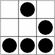
\includegraphics[width=0.5cm]{../../tarotData/img/logo_glider.png} }
\fancyfoot[LE,RO]{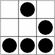
\includegraphics[width=0.5cm]{../../tarotData/img/logo_glider.png} \hfill
	\MainTitle 
\hfill \thepage /\pageref{LastPage}}
\renewcommand{\headrulewidth}{0.25pt}
\renewcommand{\footrulewidth}{0.50pt}
\addtolength{\headheight}{0.5pt}
\fancypagestyle{plain}{
	\fancyhead{}
	\renewcommand{\headrulewidth}{0pt}
}

%--- Definitions de nouvelles commandes ---
\newcommand{\N}{\mathbb{N}} % les entiers naturels

%--- Definitions de nouvelles couleurs ---
\definecolor{verylightgrey}{rgb}{0.8,0.8,0.8}
\definecolor{verylightgray}{gray}{0.80}
\definecolor{lightgrey}{rgb}{0.6,0.6,0.6}
\definecolor{lightgray}{gray}{0.6}

%============================= Corps =================================
\begin{document}

\setlength\parindent{0pt} % \noindent for all document

% \begin{longtable}[ht]{ p{4.75cm} p{0.75cm} p{4.75cm} p{0.75cm} p{4.75cm} }
\begin{longtable}[ht]{ l l l }
	%% test1 & test2 & test3 \\
	%% \hline

	\doublebox{ % \fbox{ %\Ovalbox{%
		\begin{tabular}[ht]{ @{}p{1.80cm}@{} @{}p{1.80cm}@{} @{}p{1.80cm}@{} }
			
\includegraphics[width=1.75cm, height=1.00cm]{../../tarotData/img/color_none.jpg}
				& 
\includegraphics[width=1.75cm, height=1.00cm]{../../tarotData/img/color_interrexclam.jpg}
				& 
\includegraphics[width=1.75cm, height=1.00cm]{../../tarotData/img/element_neutral.jpg} \\
			\multicolumn{3}{ @{}c@{} }{ \textbf{Arcane 0 --- Le Mat} } \\
			\multicolumn{3}{ @{}p{5.55cm}@{} }
				{ 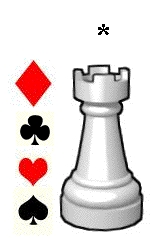
\includegraphics[width=5.50cm, height=8.00cm]{../../tarotData/img/0_Excuse_LeMat.jpg} } \\
			\multicolumn{3}{ @{}c@{} }{ \textbf{Arcane 0 --- Le Mat} } \\
			
\includegraphics[width=1.75cm, height=1.00cm]{../../tarotData/img/color_none.jpg}
				& 
\includegraphics[width=1.75cm, height=1.00cm]{../../tarotData/img/color_interrexclam.jpg}
				& 
\includegraphics[width=1.75cm, height=1.00cm]{../../tarotData/img/element_neutral.jpg} \\
		\end{tabular}
	}	&	
	\doublebox{ % \fbox{ %\Ovalbox{%
		\begin{tabular}[ht]{ @{}p{1.80cm}@{} @{}p{1.80cm}@{} @{}p{1.80cm}@{} }
			
\includegraphics[width=1.75cm, height=1.00cm]{../../tarotData/img/color_carreau.jpg}
				& 
\includegraphics[width=1.75cm, height=1.00cm]{../../tarotData/img/color_interrexclam.jpg}
				& 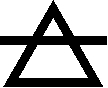
\includegraphics[width=1.75cm, height=1.00cm]{../../tarotData/img/element_air.jpg} \\
			\multicolumn{3}{ @{}c@{} }{ \textbf{Arcane I --- Le Bateleur} } \\
			\multicolumn{3}{ @{}p{5.55cm}@{} }
				{ 
\includegraphics[width=5.50cm, height=8.00cm]{../../tarotData/img/1_LeBateleur_financial.png} } \\
			\multicolumn{3}{ @{}c@{} }{ \textbf{Arcane I --- Le Bateleur} } \\
			
\includegraphics[width=1.75cm, height=1.00cm]{../../tarotData/img/color_carreau.jpg}
				& 
\includegraphics[width=1.75cm, height=1.00cm]{../../tarotData/img/color_interrexclam.jpg}
				& 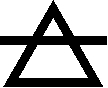
\includegraphics[width=1.75cm, height=1.00cm]{../../tarotData/img/element_air.jpg} \\
		\end{tabular}
	}	&	
	\doublebox{ % \fbox{ %\Ovalbox{%
		\begin{tabular}[ht]{ @{}p{1.80cm}@{} @{}p{1.80cm}@{} @{}p{1.80cm}@{} }
			
\includegraphics[width=1.75cm, height=1.00cm]{../../tarotData/img/color_carreau.jpg}
				& 
\includegraphics[width=1.75cm, height=1.00cm]{../../tarotData/img/color_interrexclam.jpg}
				& 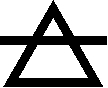
\includegraphics[width=1.75cm, height=1.00cm]{../../tarotData/img/element_air.jpg} \\
							\multicolumn{3}{ @{}c@{} }{ \textbf{Arcane II --- La Papesse} } \\
			\multicolumn{3}{ @{}p{5.55cm}@{} }
				{ 
\includegraphics[width=5.50cm, height=8.00cm]{../../tarotData/img/2_LaPapesse.jpg} } \\
			\multicolumn{3}{ @{}c@{} }{ \textbf{Arcane II --- La Papesse} } \\
			
\includegraphics[width=1.75cm, height=1.00cm]{../../tarotData/img/color_carreau.jpg}
				& 
\includegraphics[width=1.75cm, height=1.00cm]{../../tarotData/img/color_interrexclam.jpg}
				& 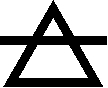
\includegraphics[width=1.75cm, height=1.00cm]{../../tarotData/img/element_air.jpg} \\
		\end{tabular}
	}	\\
	
		&	&	\\ \hline 	&	&	\\
	
	\doublebox{ % \fbox{ %\Ovalbox{%
		\begin{tabular}[ht]{ @{}p{1.80cm}@{} @{}p{1.80cm}@{} @{}p{1.80cm}@{} }
		
\includegraphics[width=1.75cm, height=1.00cm]{../../tarotData/img/color_carreau.jpg}
				& 
\includegraphics[width=1.75cm, height=1.00cm]{../../tarotData/img/color_interrexclam.jpg}
				& 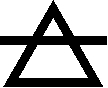
\includegraphics[width=1.75cm, height=1.00cm]{../../tarotData/img/element_air.jpg} \\
			\multicolumn{3}{ @{}c@{} }{ \textbf{Arcane III --- L'Imp{\'e}ratrice} } \\
			\multicolumn{3}{ @{}p{5.55cm}@{} }
				{ 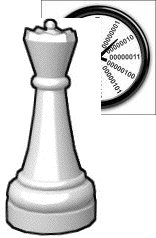
\includegraphics[width=5.50cm, height=8.00cm]{../../tarotData/img/3_LImperatrice.jpg} } \\
			\multicolumn{3}{ @{}c@{} }{ \textbf{Arcane III --- L'Imp{\'e}ratrice} } \\
			
\includegraphics[width=1.75cm, height=1.00cm]{../../tarotData/img/color_carreau.jpg}
				& 
\includegraphics[width=1.75cm, height=1.00cm]{../../tarotData/img/color_interrexclam.jpg}
				& 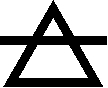
\includegraphics[width=1.75cm, height=1.00cm]{../../tarotData/img/element_air.jpg} \\
		\end{tabular}
	}	&	
	\doublebox{ % \fbox{ %\Ovalbox{%
		\begin{tabular}[ht]{ @{}p{1.80cm}@{} @{}p{1.80cm}@{} @{}p{1.80cm}@{} }
			
\includegraphics[width=1.75cm, height=1.00cm]{../../tarotData/img/color_carreau.jpg}
				& 
\includegraphics[width=1.75cm, height=1.00cm]{../../tarotData/img/color_interrexclam.jpg}
				& 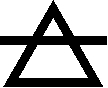
\includegraphics[width=1.75cm, height=1.00cm]{../../tarotData/img/element_air.jpg} \\
			\multicolumn{3}{ @{}c@{} }{ \textbf{Arcane IV --- L'empereur} } \\
			\multicolumn{3}{ @{}p{5.55cm}@{} }
				{ 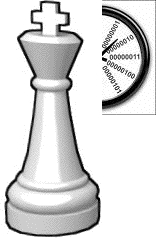
\includegraphics[width=5.50cm, height=8.00cm]{../../tarotData/img/4_LEmpereur.jpg} } \\
			\multicolumn{3}{ @{}c@{} }{ \textbf{Arcane IV --- L'empereur} } \\
			
\includegraphics[width=1.75cm, height=1.00cm]{../../tarotData/img/color_carreau.jpg}
				& 
\includegraphics[width=1.75cm, height=1.00cm]{../../tarotData/img/color_interrexclam.jpg}
				& 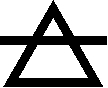
\includegraphics[width=1.75cm, height=1.00cm]{../../tarotData/img/element_air.jpg} \\
		\end{tabular}
	}	&	
	\doublebox{ % \fbox{ %\Ovalbox{%
		\begin{tabular}[ht]{ @{}p{1.80cm}@{} @{}p{1.80cm}@{} @{}p{1.80cm}@{} }
			
\includegraphics[width=1.75cm, height=1.00cm]{../../tarotData/img/color_none.jpg}
				& 
\includegraphics[width=1.75cm, height=1.00cm]{../../tarotData/img/color_interrexclam.jpg}
				& 
\includegraphics[width=1.75cm, height=1.00cm]{../../tarotData/img/element_neutral.jpg} \\
			\multicolumn{3}{ @{}c@{} }{ \textbf{Arcane V --- Le Pape} } \\
			\multicolumn{3}{ @{}p{5.55cm}@{} }
				{ 
\includegraphics[width=5.50cm, height=8.00cm]{../../tarotData/img/5_LePape.jpg} } \\
			\multicolumn{3}{ @{}c@{} }{ \textbf{Arcane V --- Le Pape} } \\
			
\includegraphics[width=1.75cm, height=1.00cm]{../../tarotData/img/color_none.jpg}
				& 
\includegraphics[width=1.75cm, height=1.00cm]{../../tarotData/img/color_interrexclam.jpg}
				& 
\includegraphics[width=1.75cm, height=1.00cm]{../../tarotData/img/element_neutral.jpg} \\
		\end{tabular}
	}	\\
	
		&	&	\\ \hline 	&	&	\\
	
	\clearpage
	
	\doublebox{ % \fbox{ %\Ovalbox{%
		\begin{tabular}[ht]{ @{}p{1.80cm}@{} @{}p{1.80cm}@{} @{}p{1.80cm}@{} }
			\multicolumn{3}{ @{}p{5.55cm}@{} }
				{ 
\includegraphics[width=5.50cm, height=11.25cm]{../../tarotData/img/cards_background.jpg} } \\
		\end{tabular}
	}	&	
	\doublebox{ % \fbox{ %\Ovalbox{%
		\begin{tabular}[ht]{ @{}p{1.80cm}@{} @{}p{1.80cm}@{} @{}p{1.80cm}@{} }
			\multicolumn{3}{ @{}p{5.55cm}@{} }
				{ 
\includegraphics[width=5.50cm, height=11.25cm]{../../tarotData/img/cards_background.jpg} } \\
		\end{tabular}
	}	&	
	\doublebox{ % \fbox{ %\Ovalbox{%
		\begin{tabular}[ht]{ @{}p{1.80cm}@{} @{}p{1.80cm}@{} @{}p{1.80cm}@{} }
			\multicolumn{3}{ @{}p{5.55cm}@{} }
				{ 
\includegraphics[width=5.50cm, height=11.25cm]{../../tarotData/img/cards_background.jpg} } \\
		\end{tabular}
	}	\\
	
		&	&	\\ \hline 	&	&	\\
		
	\doublebox{ % \fbox{ %\Ovalbox{%
		\begin{tabular}[ht]{ @{}p{1.80cm}@{} @{}p{1.80cm}@{} @{}p{1.80cm}@{} }
			\multicolumn{3}{ @{}p{5.55cm}@{} }
				{ 
\includegraphics[width=5.50cm, height=11.25cm]{../../tarotData/img/cards_background.jpg} } \\
		\end{tabular}
	}	&	
	\doublebox{ % \fbox{ %\Ovalbox{%
		\begin{tabular}[ht]{ @{}p{1.80cm}@{} @{}p{1.80cm}@{} @{}p{1.80cm}@{} }
			\multicolumn{3}{ @{}p{5.55cm}@{} }
				{ 
\includegraphics[width=5.50cm, height=11.25cm]{../../tarotData/img/cards_background.jpg} } \\
		\end{tabular}
	}	&	
	\doublebox{ % \fbox{ %\Ovalbox{%
		\begin{tabular}[ht]{ @{}p{1.80cm}@{} @{}p{1.80cm}@{} @{}p{1.80cm}@{} }
			\multicolumn{3}{ @{}p{5.55cm}@{} }
				{ 
\includegraphics[width=5.50cm, height=11.25cm]{../../tarotData/img/cards_background.jpg} } \\
		\end{tabular}
	}	\\
	
		&	&	\\ \hline 	&	&	\\
		
	%% \clearpage
	
\end{longtable}

\end{document}
